\begin{enumerate}[label=\thechapter.\arabic*,ref=\thechapter.\theenumi]
\item The value of the contour integral, $\oint_C \frac{z + 2}{z^2 + 2z + 2} \, dz$, where the contour $C$ is $\{ z : |z + 1 - \frac{3}{2}i| = 1 \}$, taken in the counter clockwise direction, is \\

\begin{enumerate}
  \item[(A)] $-\pi(1+j) $
  \item[(B)] $\pi(1+j)$
  \item[(C)] $\pi(1-j) $
  \item[(D)] $-\pi(1-j)$
\end{enumerate}

\hfill{(GATE EC 2023)}\\
\solution
\documentclass[journal,12pt,twocolumn]{IEEEtran}

% Packages
\usepackage{cite}
\usepackage{amsmath,amssymb,amsfonts,amsthm}
\usepackage{graphicx}
\usepackage{textcomp}
\usepackage{xcolor}
\usepackage{txfonts}
\usepackage{listings}
\usepackage{enumitem}
\usepackage{mathtools}
\usepackage{float}
\usepackage{gensymb}
\usepackage{comment}
\usepackage{hyperref}
\usepackage{tkz-euclide}
\usepackage{gvv}
\usepackage[latin1]{inputenc}
\usepackage{color}
\usepackage{array}
\usepackage{longtable}
\usepackage{calc}
\usepackage{multirow}
\usepackage{hhline}
\usepackage{ifthen}
\usepackage{lscape}
\usepackage{subcaption}
\usepackage{tikz}
\usepackage{circuitikz}
\usepackage{wrapfig}
\usepackage{lipsum}
\usepackage[export]{adjustbox}
\usepackage{inputenc}

% Custom commands and macros
\newtheorem{theorem}{Theorem}[section]
\newtheorem{problem}{Problem}
\newtheorem{proposition}{Proposition}[section]
\newtheorem{lemma}{Lemma}[section]
\newtheorem{corollary}[theorem]{Corollary}
\newtheorem{example}{Example}[section]
\newtheorem{definition}[problem]{Definition}
\newtheorem{rem}{Remark}
\newcommand{\BEQA}{\begin{eqnarray}}
\newcommand{\EEQA}{\end{eqnarray}}
\newcommand{\define}{\stackrel{\triangle}{=}}
\renewcommand{\thefigure}{\theenumi}
\renewcommand{\thetable}{\theenumi}



\begin{document}

\title{GATE 2023 EC 49}
\author{EE23BTECH11045 - Palavelli Srija$^{*}$}
\maketitle

\bigskip

\textbf{Question 12.7.7:} 
Let $x(t) = 10 \cos(10.5 \omega t)$ be passed through an LTI system with impulse response $h(t) = \pi\left(\frac{\sin(\omega t)}{\pi t}\right)^2 \cos(10 \omega t)$ . The output of the system is: \\

\textbf{Solution:}
\begin{table}[h!]
    \centering
    \begin{table}[htbp]
	\centering
	\noindent
	\fontsize{10}{15}\selectfont {
		\resizebox{0.45\textwidth}{!}{%
			\begin{tabular}{|c|c|c|}
				\hline
				\textbf{Parameter} & \textbf{Value} & \textbf{Description} \\
				\hline
				$x\brak t$ & - & Input voltage \\
				\hline
				$y\brak t$ & - & Output voltage \\
				\hline
				$h\brak t$ & $\frac{y\brak t}{x\brak t}$ & Impulse response \\
				\hline
				$X\brak s$ & - & Input voltage in s-domain \\
				\hline
				$Y\brak s$ & - & Output voltage in s-domain \\
				\hline
				$H\brak s$ & $\frac{Y\brak s}{X\brak s}$ & Impulse response in s-domain \\
				\hline
			\end{tabular}
	} }
	\caption*{Input Table}
	
\end{table}
    \caption{Input Parameters}
    \label{tab:table_sr10}
\end{table}

Given \(h(t)\) is real and even. When a sinusoidal input is applied to an LTI system with an even impulse response, the output will also be sinusoidal. Hence, \(y(t) = A\cdot 10\cos(10.5 \omega t + \theta)\).

\[
x(t) \xrightarrow{\text{}} \boxed{\text{h(t)}} \xrightarrow{\text{}} y(t)
\]

\begin{align}
\text{Let } f(t) &= \pi\left(\frac{\sin(\omega t)}{\pi t}\right)^2 \\
h(t) &= f(t) \cos(10 \omega t)
\end{align}

Using 
\begin{align}
x_1(t) \cdot x_2(t) \xleftrightarrow{\mathcal{F}} X_1(\omega) * X_2(\omega)\\
\left(\frac{\sin(\omega t)}{\pi t}\right) \cdot \left(\frac{\sin(\omega t)}{\pi t}\right) \xleftrightarrow{\mathcal{F}} X_1(\omega) * X_2(\omega)
\end{align}
\begin{figure}[h!]
    \centering
    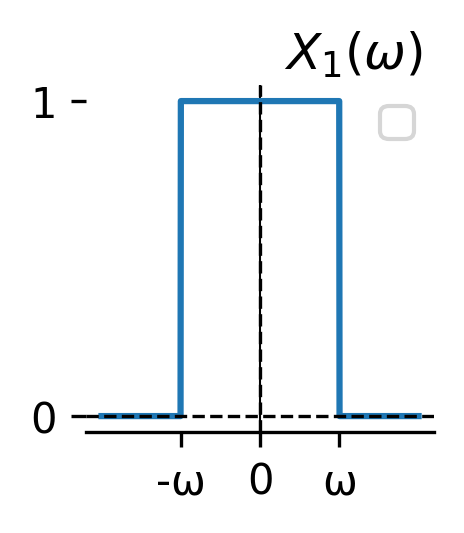
\includegraphics[width=0.4\columnwidth, height=2.5cm]{figs/plot.png}\hfill
    \begin{tabular}{c}
        {\sffamily\raisebox{1.75cm}{*}} 
    \end{tabular}\hfill
    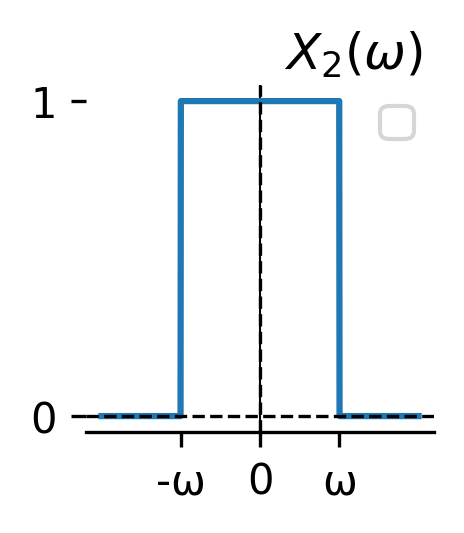
\includegraphics[width=0.4\columnwidth, height=2.5cm]{figs/plot4.png}
    
    \caption{}
    \label{fig:overall}
\end{figure}

\begin{align}
\left(\frac{\sin(\omega t)}{\pi t}\right)^2  \xleftrightarrow{\mathcal{F}} X_3(\omega) 
\end{align}
\begin{figure}[h!]
    \centering
    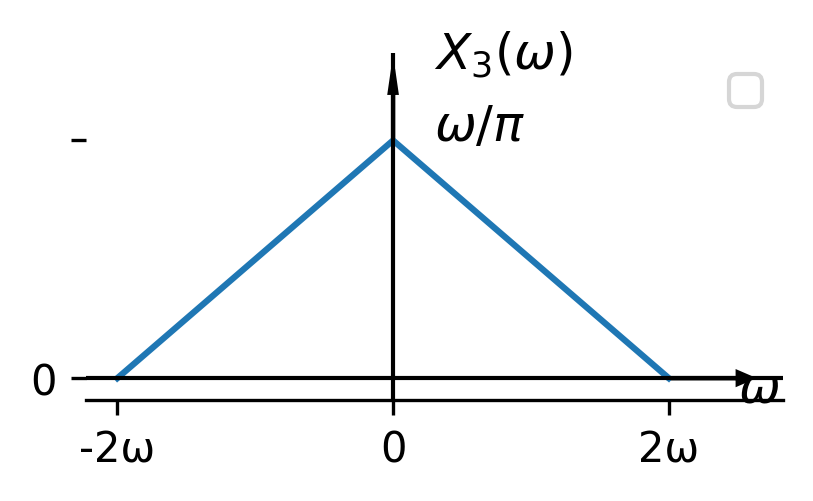
\includegraphics[width=0.5\columnwidth, height=3cm]{figs/plot1.png}
    \caption{}
    \label{fig:sr11}
\end{figure}
\begin{align}
\pi\left(\frac{\sin(\omega t)}{\pi t}\right)^2 \xleftrightarrow{\mathcal{F}} X_4(\omega)
\end{align}
\begin{figure}[h!]
    \centering
    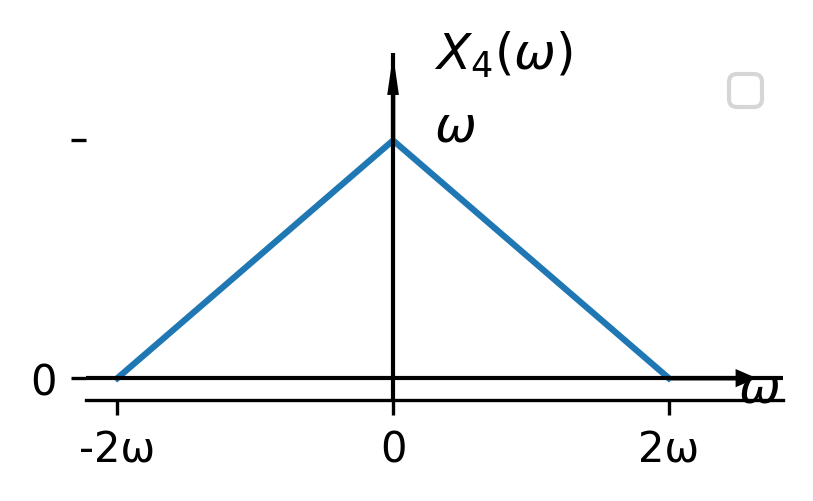
\includegraphics[width=0.5\columnwidth, height=3cm]{figs/plot2.png}
    \caption{}
    \label{fig:sr12}
\end{figure}
    \begin{align}
\text{From modulating property:} \nonumber \\
        f(t) \cos(\omega_0 t) \xleftrightarrow{\mathcal{F}} \frac{1}{2} \left[F(\omega + \omega_0) + F(\omega - \omega_0)\right]
    \end{align}

    \begin{align}
        H(\omega) &= \frac{1}{2} \left[F(\omega + 10\omega) + F(\omega - 10\omega)\right]
    \end{align}

\begin{figure}[h!]
    \centering
    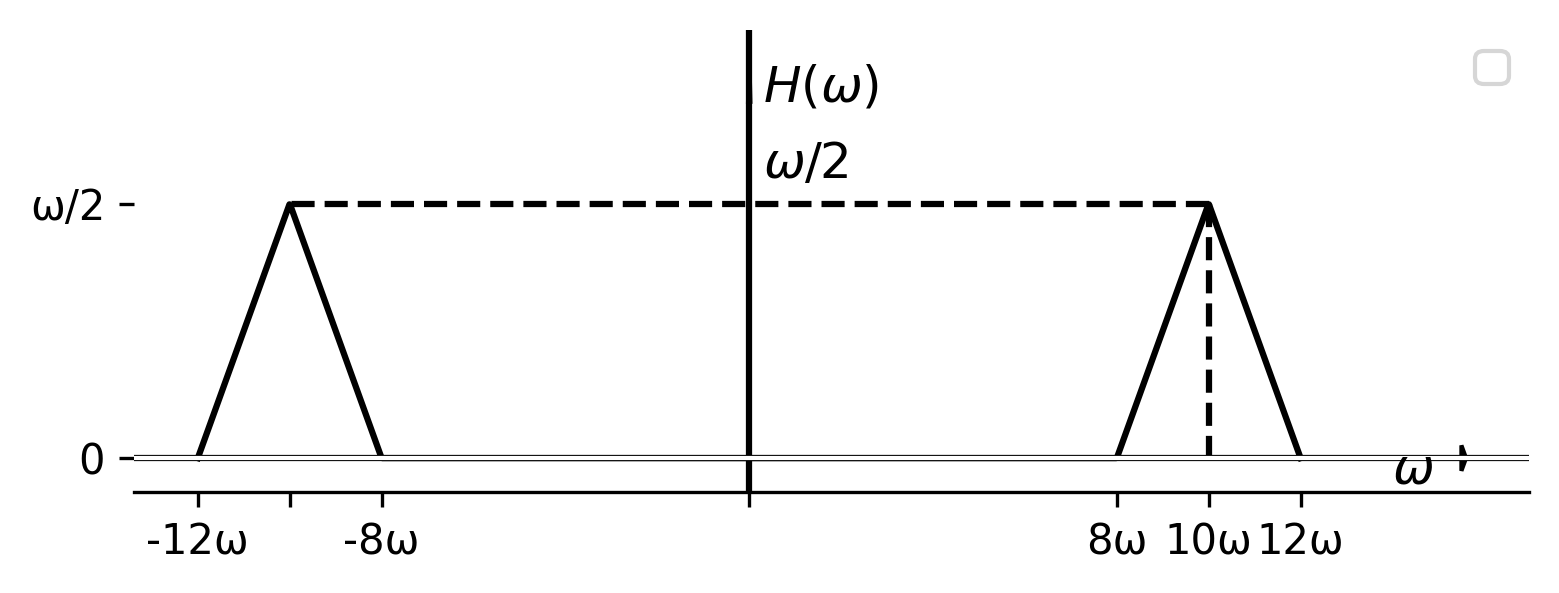
\includegraphics[width=0.7\columnwidth,height=2.5cm]{figs/plot3.png}
    \caption{}
    \label{fig:sr13}
\end{figure}
\begin{equation}
    \frac{\frac{\omega}{2} - 0}{10\omega - 12\omega} = \frac{|H(10.5\omega)| - 0}{10.5\omega - 12\omega}
\end{equation}

\begin{align}
A = |H(10.5\omega)| &= \frac{3}{8}\omega \quad \text{and} \quad  \theta= \angle H(10.5\omega) = 0^\circ
\end{align}

The output \(y(t)\):
\begin{align}
y(t) &= \frac{3}{8}\omega \cdot 10 \cos(10.5 \omega t) \\
&= \frac{15}{4}\omega \cos(10.5 \omega t)
\end{align}
\begin{figure}[h!]
    \centering
    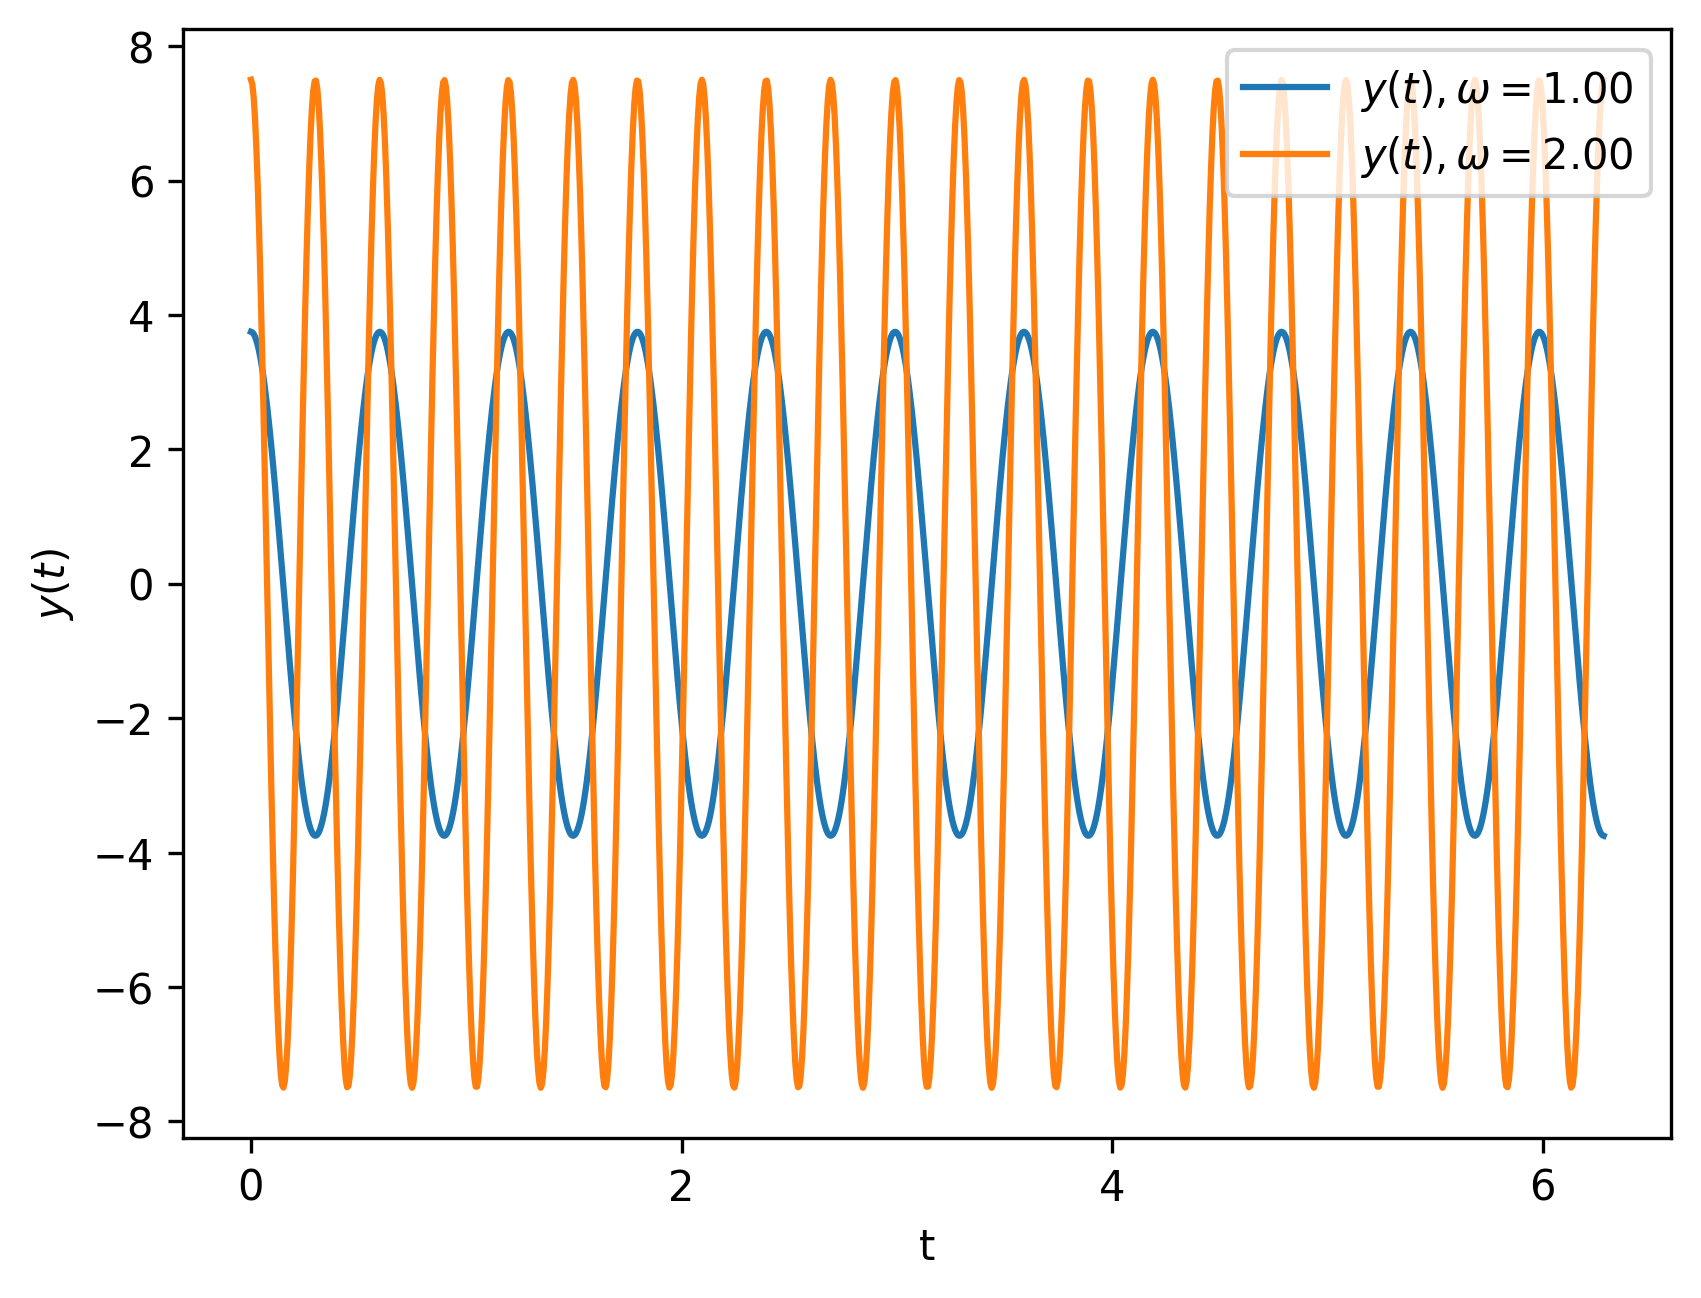
\includegraphics[width=\columnwidth]{figs/plot5.png}
    \caption{}
    \label{fig:sr14}
\end{figure}
\end{document}


\pagebreak

\item The function $f(z)=\frac{1}{z-1}$ of a complex variable z is integrated on a closed contour in an anti-clockwise direction. For which of the following contours, does this integral have a non-zero value?\\
\brak{A}$\abs{z-2}=0.01$\\
\brak{B}$\abs{z-1}=0.1$\\
\brak{C}$\abs{z-3}=5$\\
\brak{D}$\abs{z}=2$\\
\hfill(GATE 2023 BM)\\
\solution
\iffalse
\let\negmedspace\undefined
\let\negthickspace\undefined
\documentclass[journal,12pt,twocolumn]{IEEEtran}
\usepackage{cite}
\usepackage{amsmath,amssymb,amsfonts,amsthm}
\usepackage{algorithmic}
\usepackage{graphicx}
\usepackage{textcomp}
\usepackage{xcolor}
\usepackage{txfonts}
\usepackage{listings}
\usepackage{enumitem}
\usepackage{mathtools}
\usepackage{gensymb}
\usepackage{comment}
\usepackage[breaklinks=true]{hyperref}
\usepackage{tkz-euclide} 
\usepackage{listings}
\usepackage{gvv}                                        
\def\inputGnumericTable{}                                 
\usepackage[latin1]{inputenc}                                
\usepackage{color}                                            
\usepackage{array}                                            
\usepackage{longtable}                              
\usepackage{calc}                                             
\usepackage{multirow}                                         
\usepackage{hhline}                                           
\usepackage{ifthen}                                           
\usepackage{lscape}

\newtheorem{theorem}{Theorem}[section]
\newtheorem{problem}{Problem}
\newtheorem{proposition}{Proposition}[section]
\newtheorem{lemma}{Lemma}[section]
\newtheorem{corollary}[theorem]{Corollary}
\newtheorem{example}{Example}[section]
\newtheorem{definition}[problem]{Definition}
\newcommand{\BEQA}{\begin{eqnarray}}
\newcommand{\EEQA}{\end{eqnarray}}
\newcommand{\define}{\stackrel{\triangle}{=}}
\theoremstyle{remark}
\newtheorem{rem}{Remark}
\begin{document}

\bibliographystyle{IEEEtran}
\vspace{3cm}

\title{GATE 2023}
\author{EE23BTECH11020 - Raghava Ganji$^{*}$% <-this % stops a space
}
\maketitle
\newpage
\bigskip

\renewcommand{\thefigure}{\theenumi}
\renewcommand{\thetable}{\theenumi}

\textbf{GATE 2023 BM.48:}
The function $f(z)=\frac{1}{z-1}$ of a complex variable z on a closed contour in an anti-clockwise direction.For which of the following contours, does this integral have a non-zero value?\\
\brak{A}$\abs{z-2}=0.01$\\
\brak{B}$\abs{z-1}=0.1$\\
\brak{C}$\abs{z-3}=5$\\
\brak{D}$\abs{z}=2$\\
\solution\\
\fi
Cauchy's Integral Formula and Residue Theorem.
\begin{align}
\oint_{c}f\brak z&=2\pi jRes\sbrak{f\brak z,z_0}\label{eq:CIF}\\
Res\sbrak{f\brak z,z_0}&=\lim_{z\to z_0}\sbrak{\brak{z-z_0}f\brak z}\label{eq:Res Thm}
\end{align}
Here $z_0$ is pole of the f\brak z\\
Using \eqref{eq:CIF}
\begin{align}
\oint_{c}\frac{1}{z-1}dz &=2\pi jRes\sbrak{\frac{1}{z-1},1}
\end{align}
\begin{enumerate}
\item For option A the pole is outside the contour, then Residue is zero.\\
\begin{figure}[h!]
    \centering
    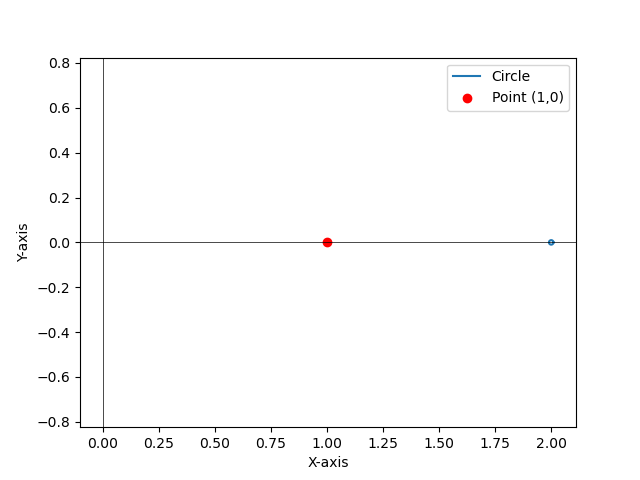
\includegraphics[width=1\columnwidth]{2023/BM/48/figs/plotg231.png}
    \caption{graph of option A}
\end{figure}
\begin{align}
\implies\oint_{c}\frac{1}{z-1}dz &=2\pi j\brak{0}\\
\implies 0
\end{align}
\item For option B the pole is inside the contour.\\
\begin{figure}[h!]
    \centering
    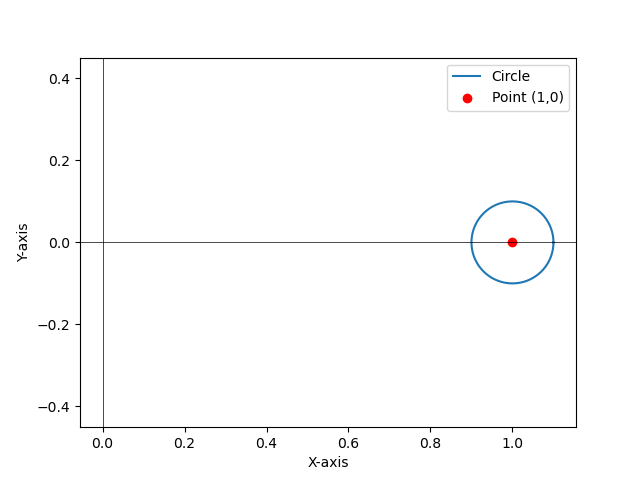
\includegraphics[width=1\columnwidth]{2023/BM/48/figs/plotg232.png}
    \caption{graph of option B}
\end{figure}
Then, using \eqref{eq:Res Thm}
\begin{align}
Res\sbrak{\frac{1}{z-1},1} &=\lim_{z\to 1}\brak{z-1}\frac{1}{z-1}\\
&=1\\
\implies \oint_{c}\frac{1}{z-1}dz&=2\pi j\brak 1\\
\implies 2\pi j
\end{align}
\item For option C the pole is inside the contour.\\
\begin{figure}[h!]
    \centering
    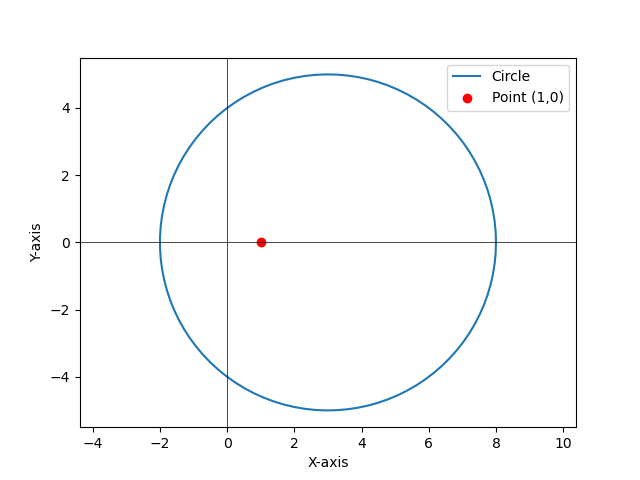
\includegraphics[width=1\columnwidth]{2023/BM/48/figs/plotg233.png}
    \caption{graph of option C}
\end{figure}
Then, using \eqref{eq:Res Thm}
\begin{align}
Res\sbrak{\frac{1}{z-1},1} &=\lim_{z\to 1}\brak{z-1}\frac{1}{z-1}\\
&=1\\
\implies \oint_{c}\frac{1}{z-1}dz&=2\pi j\brak 1\\
\implies 2\pi j
\end{align}
\item For option D the pole is inside the contour.\\
\begin{figure}[h!]
    \centering
    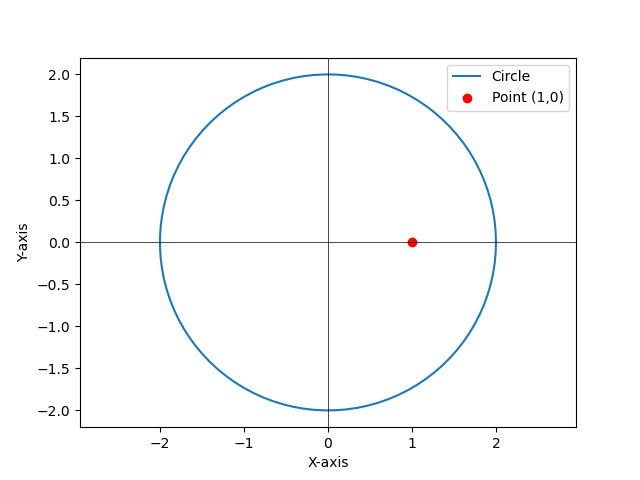
\includegraphics[width=1\columnwidth]{2023/BM/48/figs/plotg234.png}
    \caption{graph of option D}
\end{figure}
Then, using \eqref{eq:Res Thm}
\begin{align}
Res\sbrak{\frac{1}{z-1},1} &=\lim_{z\to 1}\brak{z-1}\frac{1}{z-1}\\
&=1\\
\implies \oint_{c}\frac{1}{z-1}dz&=2\pi j\brak 1\\
\implies 2\pi j
\end{align}
\end{enumerate}
We can conclude that for options B,C,D contours have the non-zero value for this integral.
%\end{document}

\newpage
\item Consider the contour integral $\oint \frac{dz}{z^4 + z^3 - 2z^2}$, along the curve $|z| = 3$ oriented in the counterclockwise direction. If $\text{Res}[f, z_0]$ denotes the residue of $f(z)$ at the point $z_0$, then which of the following are TRUE? \\
\begin{itemize}
    \item (A) $\text{Res}[f, 0] = -\frac{1}{4}$
    \item (B) $\text{Res}[f, 1] = \frac{1}{3}$
    \item (C) $\text{Res}[f, -2] = -\frac{1}{12}$
    \item (D) $\text{Res}[f, 2] = -1$
\end{itemize}
\hfill{(GATE NM 2023)}\\
\solution
\newpage
\end{enumerate}
